\documentclass[11pt]{article}
\usepackage{graphicx}
\usepackage{array}
\usepackage{booktabs}
\usepackage[a4paper,margin=3cm, headheight=90pt]{geometry}
\usepackage{cmbright}
\usepackage[OT1]{fontenc}
\usepackage{float}
\usepackage[table]{xcolor}
\usepackage{pgfplots}
\pgfplotsset{compat=newest}
\usepackage{caption}
\usepackage{subcaption}
\usepackage{fancyhdr}
\usepackage{blindtext}
\usepackage{natbib}
\setcitestyle{square}
\usepackage{url}
\usepackage{wrapfig}
\usepackage{amsmath}
\usepackage{parskip}
\usepackage{tabularx}
\newcolumntype{Y}{>{\centering\arraybackslash}X}
\usepackage{multirow}

\title{\vspace{-2cm}
\includegraphics[width=0.3\textwidth]{/Users/finn/Documents/Cardiff-University-logo-for-website}~\\[1cm]
Classification of the abnormal globular cluster NGC 3201 
}
\author{Finnbar Wilson - 22031076}
\date{\today}

\begin{document}

\maketitle

\section*{Abstract}

NGC 3201 is an abnormal globular cluster due to its inhomogeneous stellar population and has been classified as a young halo, which has an extragalactic origin, by \citet{Mackey}. The classification scheme by \citet{Mackey} does not take into account the differences that an abnormal cluster may have compared to a regular globular cluster. In this report a colour magnitude diagram of NGC 3201 was made in the B and V filters so that isochrone can be fitted to determine the age and metallicity of NGC 3201. The age was found to be 12.0 Gyr and its metallicity to be [M/H] $=-0.4$. This age is inline with current values for NGC 3201's age but it's metallicity is not. Further analysis of the ages of stellar populations within the cluster found that NGC 3201 might have been formed from the merger between two previous globular clusters. All results found in this report suggests that NGC 3201 is galactic in origin which is in disagreement with \citet{Mackey}.

\pagebreak
\section{Introduction}

NGC 3201 is a globular cluster, discovered by James Dunlop on the 28th of May 1826, located at 10$^{\text{h}}$ 17$^{\text{m}}$ 36.82$^{\text{s}}$/-46$^{\circ}$ 24' 44.9" (in RA/Dec) 5.0 kpc away from the Sun \citep{3201fact}. NGC 3201 has a large sub-cluster of black holes in its core making it an interesting source for observing the interactions in large populations of black holes \citep{blackholes}.

\begin{figure}[h]
	\centering
	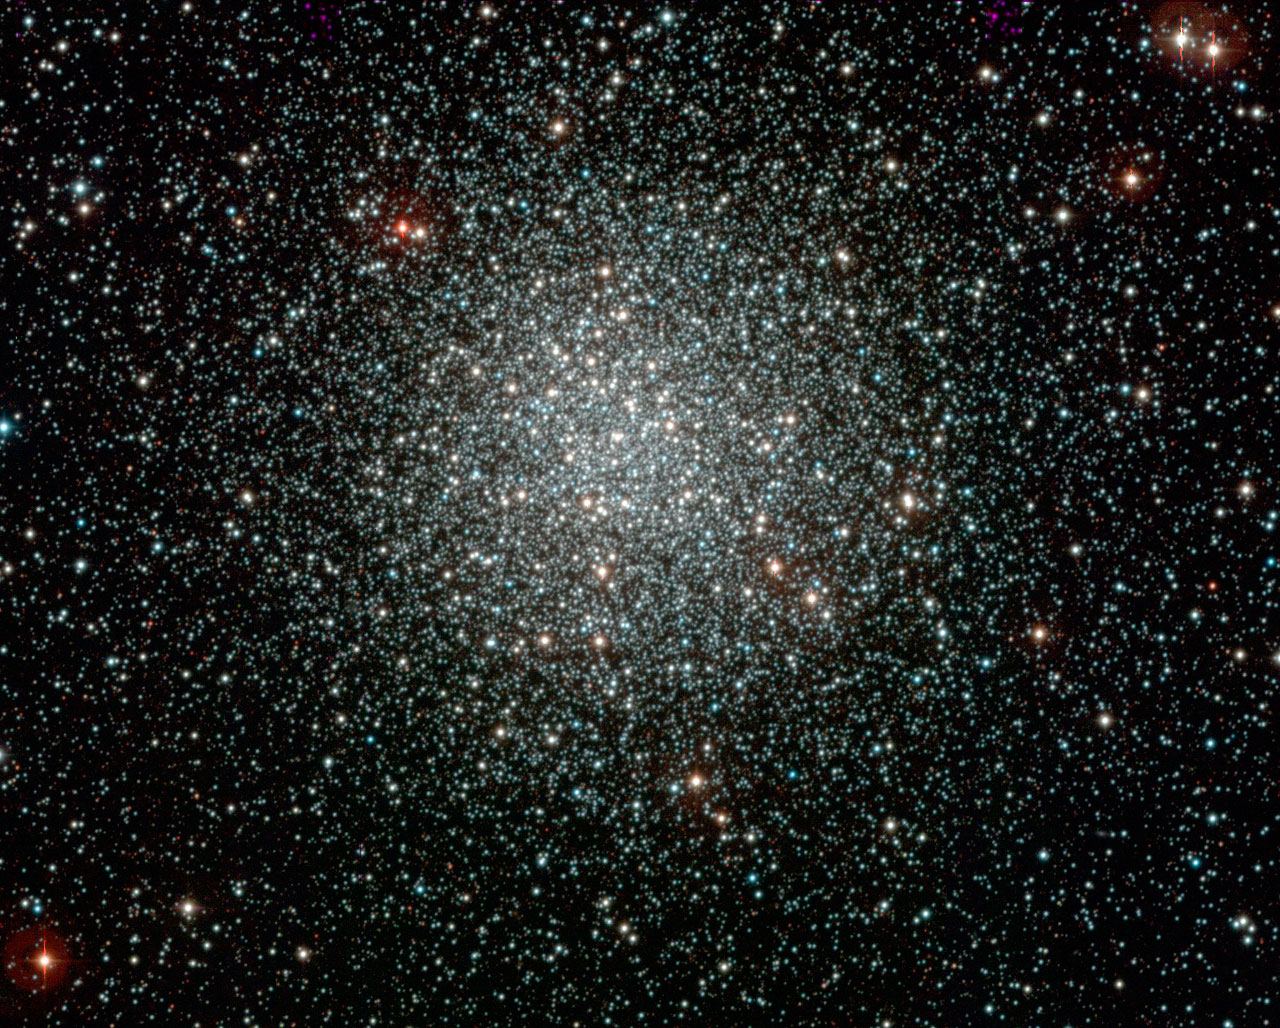
\includegraphics[width=0.4\textwidth]{../Figures/NGC3201}
	\caption{Picture of NGC 3201 by Hubble Space Telescope \citep{image}}
\end{figure}

Globular clusters are among the oldest stellar populations in the universe, providing key insights into how stars and galactic structures evolve. In the Milky Way, some globular clusters are thought to have originated outside the galaxy due to their similar properties to satellite dwarf galaxies, whereas others are believed to have evolved within the milky way itself due to the observable effects of tidal forces and shocks in the inner galaxy. This allows for globular clusters to be classified by their characteristics as shown by \citet{Mackey} into three types: 'Young' halo(YH) which are thought to have been formed in external galaxies, 'Old' halo(OH) and 'Bulge/Disc'(BD) which are formed in the milky way. According to \citet{Mackey}, their study on globular clusters classified NGC 3201 as a YH cluster based on the metallicity and redder horizontal branch stars. NGC 3201 stands out from other clusters classified by \citet{Mackey} due to its irregular radial velocity and differential reddening across its face \citep{Kravtsov}. This makes it one of the few known clusters with an inhomogeneous stellar population for its size, which could affect how it has been classified.

In this report the structure of NGC 3201 will be analysed by finding the stellar populations inside the cluster and comparing them to isochrones to determine their age. These stellar populations will then allow a greater insight into the internal structure of the cluster creating a more actuate analysis of its classification. Given that NGC 3201 is an abnormal cluster this report will also test various methods of determining the classification of abnormal clusters.

\pagebreak
\section{Procedure}

\subsection{Calibration}

Two images of NGC 3201 were taken in the V and B filters on a 1.0m diameter telescope. Five stars were found in each filter to calibrate the zero point magnitude in each image and their data can be found in Table \ref{tab:calB} \& \ref{tab:calV}. To find the calibration stars, a catalog of local stars from \citet{simbad} was overlaid in each image and 10 stars were selected in total and their known magnitudes recored. An aperture photometry of each star was performed and recorded, as well as their error.

\begin{table}[H]
\centering
\caption{Calibration stars in B filter}
\begin{tabular}{lccccc}
\toprule
ID & RA & Dec & B$_{\text{instrument}}$ & B$_{\text{simbad}}$ \\
\midrule
Cl* NGC 3201 CWFD 3-109 &  10:17:23.65 &  -46:24:17.31 & -12.566$\pm 0.004$ & 16.216 \\                  
Cl* NGC 3201 CWFD 3-198 &  10:17:34.49 &  -46:25:36.15 & -12.947$\pm 0.003$ & 15.800 \\                 
Cl* NGC 3201 CWFD 3-224 &  10:17:36.86 &  -46:23:11.97 & -15.062$\pm 0.001$ & 13.601 \\                 
NGC 3201 3401 &  10:17:38.12 &  -46:22:39.29 & -14.787$\pm 0.001$ & 14.080 \\                           
NGC 3201 4319 &  10:17:42.55 &  -46:27:15.42 & -14.812$\pm 0.001$ & 13.999 \\
\bottomrule
\end{tabular}
\caption*{ID is the stars identification searchable on the SIMBAD database, B$_{\text{instrument}}$ is the magnitude recorded in this experiment and B$_{\text{simbad}}$ is the known magnitude found on SIMBAD \citep{simbad}}
\label{tab:calB}
\end{table}

\begin{table}[h]
\centering
\caption{Calibration stars in V filter}
\begin{tabular}{lcccccc}
\toprule
ID & RA & Dec & V$_{\text{instrument}}$ & V$_{\text{simbad}}$\\
\midrule
2MASS J10173339-4620241 & 10:17:33.39 & -46:20:24.16 & -13.579$\pm 0.003$ & 15.650 \\                   
Cl* NGC 3201 CWFD 3-296 & 10:17:42.26 & -46:19:47.92 & -13.904$\pm 0.002$ & 15.230 \\                  
Cl* NGC 3201 CWFD 3-255 & 10:17:38.86 & -46:22:56.86 & -14.536$\pm 0.002$ & 14.730 \\                  
Cl* NGC 3201 CWFD 3-235 & 10:17:37.72 & -46:22:53.50 & -14.410$\pm 0.002$ & 14.910 \\                     
Cl* NGC 3201 CWFD 3-195 & 10:17:34.01 & -46:23:26.20 & -13.225$\pm 0.003$ & 16.030\\ 
\bottomrule
\end{tabular}
\caption*{ID is the stars identification searchable on the SIMBAD database, V$_{\text{instrument}}$ is the magnitude recorded in this experiment and V$_{\text{simbad}}$ is the known magnitude found on SIMBAD \citep{simbad}}
\label{tab:calV}
\end{table}

The equation to find the zero point magnitude is shown by Equation \ref{eq:zp}.
\begin{equation}
	m_{\text{zero point}} = m_{\text{simbad}} - m_{\text{instrument}}
	\label{eq:zp}
\end{equation}
Where $m$ is the magnitude (B or V). This produced a zero point magnitude of: B$_{\text{zero point}} = 28.774 \pm 0.005$ and V$_{\text{zero point}} = 29.2407 \pm 0.0010$. The errors associated with these values are from the error in the $m_{\text{instrument}}$ recordings as well as the error in the $m_{\text{simbad}}$ which are not shown in Table \ref{tab:calB} \& \ref{tab:calV} but can be found on \citet{simbad}. 

\subsection{Automated detection}

An object detection tool from \citet{gaia} was used to quickly identify the magnitudes of large number of stars in each image as well as their positions and information on how they selected those stars. These two large datasets were then uploaded into \citet{topcat} which matched the two filters by their positions so that the magnitudes recorded are for the same stars. This matched dataset can be found on the \citet{github}. The automated object detection tool found it hard to identify singular stars in the dense core so other detection methods are needed to analyse the central stars of the cluster. This tool was able to calculate the error in both magnitudes. This method records magnitude as apparent magnitude so to convert it into absolute magnitude Equation \ref{eq:absolute} can be used.
\begin{equation}
	m-M = 5 \log \left( \frac{d}{10} \right)
	\label{eq:absolute}
\end{equation}
Where $m$ is the apparent magnitude, $M$ is the absolute magnitude and $d$ is the distance to NGC 3201.
\subsection{Manual detection}

An aperture photometry tool was used to manually determine the magnitude of stars focusing especially around the core where the automated detections system found it harder to detect stars. Stars were chosen based on their shape, to ensure only singular stars were recored instead of multiple, as well as their brightness. This tool was able to calculate the error in the magnitude data for both filters. In total 80 stars were recorded.

\pagebreak
\section{Analysis}

\subsection{Determining age of NGC 3201}

The matched data from the automated detection method is shown in Figure \ref{fig:origin}. The matched dataset originally recored 7612 stars but this number was reduced to 2411 stars by removing stars that lay outside of 0.152$^{\circ}$ from the centre of the cluster as this is the radius of NGC3201 \citep{radius}. 

\begin{figure}[H]
	\centering
	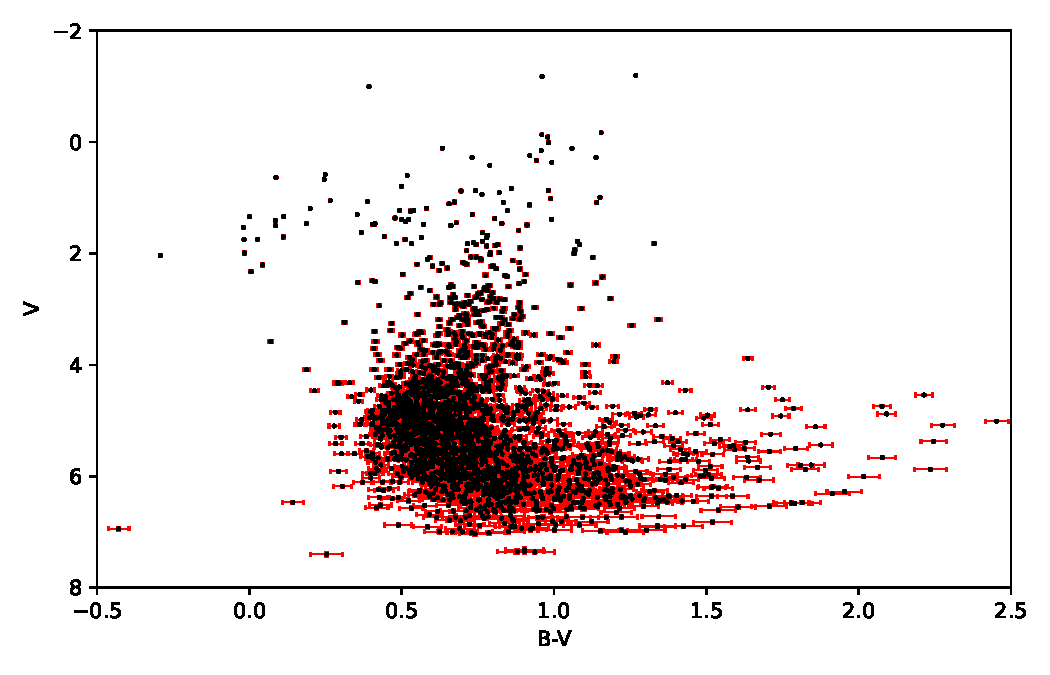
\includegraphics[width=0.8\textwidth]{../Figures/errobar}
	\caption{Colour magnitude diagram in the B and V filters from the matched dataset. The absolute magnitude in the V filter is shown on the y axis and the B magnitude minus V magnitude is shown on the x axis. Each data point has an error which is shown by the red error bars.}
	\label{fig:origin}
\end{figure}

To determine the age of NGC 3201, several isochrones from \citet{iso} with different metallicities were plotted onto the colour magnitude diagram shown in Figure \ref{fig:isomany}. From these plotted isochrones, an age and metallicity that most closely matched the main sequence turn off from the data recorded was chosen. This isochrone, which is plotted in Figure \ref{fig:singiso}, has an [M/H] $= -0.4$ and Age of 12 Gyr. 

\begin{figure}[H]
	\centering
	\begin{subfigure}[b]{0.49\textwidth}
		\centering
		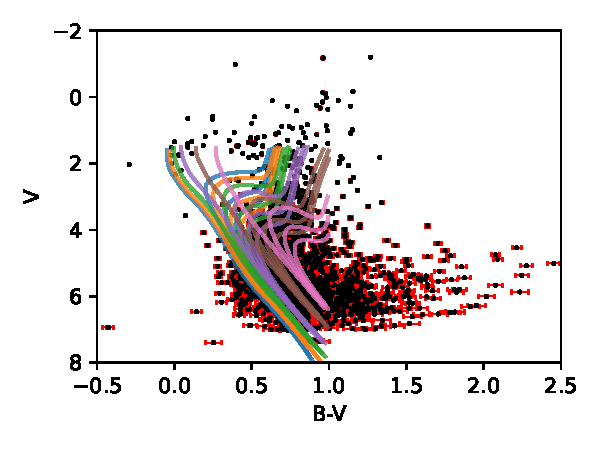
\includegraphics[width=\textwidth]{../Figures/manyiso}
		\caption{}
		\label{fig:isomany}
	\end{subfigure}
	\hfill
	\begin{subfigure}[b]{0.49\textwidth}
		\centering
		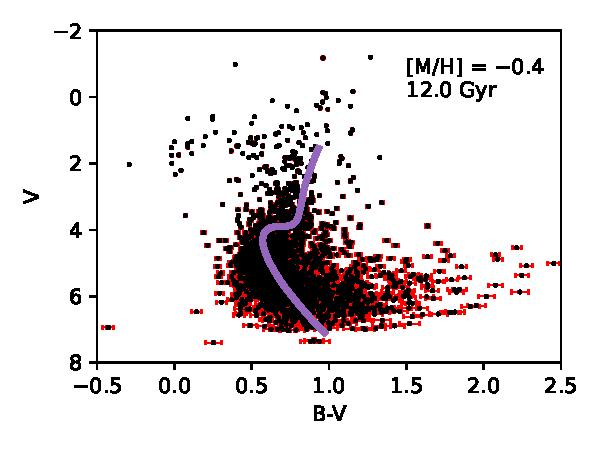
\includegraphics[width=\textwidth]{../Figures/singiso}
		\caption{}
		\label{fig:singiso}
	\end{subfigure}
	\caption{Two colour magnitude diagrams in B and V filters. \ref{fig:isomany} has several isochrones with ranging metallicity ([M/H]), shown by colour, and age. The [M/H] attached to each colour is: Blue $= -1.8$, Orange $= -1.4$, Green $= -1.0$, Purple $= -0.4$, Brown $= -0.2$, Pink $= 0.2$. The isochrone with the best fit is shown in \ref{fig:singiso} has a [M/H] $=-0.4$ and an age of 12.0 Gyr. }
	\label{fig:iso}
\end{figure}

The data recorded from the manual aperture photometry is shown in Table \ref{tab:manual}. The results have been converted to Absolute magnitude using Equation \ref{eq:absolute} and a plot of the data recorded is shown in Figure \ref{fig:man}. Also plotted on Figure \ref{fig:man} is the best matched isochrone found in the automatic detection method.

\begin{figure}[h]
	\centering
	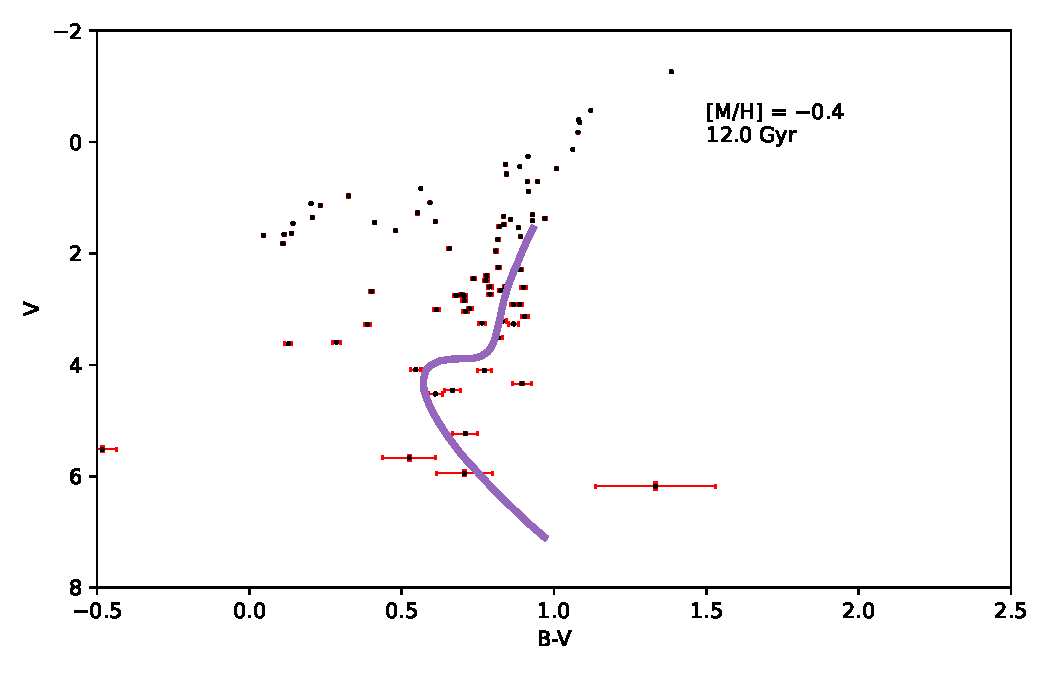
\includegraphics[width=0.8\textwidth]{../Figures/manual}
	\caption{A colour magnitude diagram of the stars recorded using the manual aperture photometry tool. Also shown is the isochrone from the automatic detection method shown in purple. In total 80 stars were recorded. }
	\label{fig:man}
\end{figure}

The isochrone in Figure \ref{fig:man} is not a good fit to the stars so further analysis of the metallicity and age of the manually detected stars is shown in section 3.2 were it is referred to as 'Core stars'.

\newgeometry{left=1cm,right=1cm,bottom=3cm,top=3cm}

\begin{table}
\caption{Manual aperture photometry results}

\begin{minipage}{0.48\paperwidth}
\centering
\begin{tabular}{cccccc}
\toprule
RA$^{\circ}$ & Dec$^{\circ}$ & B & B$_{err}$ & V & V$_{err}$ \\
\midrule
154.356 & -46.379 & 2.032 & 0.003 & 1.422 & 0.002 \\
154.381 & -46.393 & 1.305 & 0.002 & 1.103 & 0.002 \\
154.411 & -46.390 & 0.900 & 0.002 & -0.179 & 0.001 \\
154.404 & -46.403 & 3.263 & 0.007 & 2.486 & 0.004 \\
154.388 & -46.413 & 1.417 & 0.002 & 0.573 & 0.001 \\
154.409 & -46.406 & 1.720 & 0.003 & 1.673 & 0.002 \\
154.411 & -46.413 & 2.764 & 0.005 & 1.955 & 0.003 \\
154.400 & -46.423 & 2.340 & 0.004 & 1.370 & 0.002 \\
154.401 & -46.411 & 6.197 & 0.091 & 15.746 & 100.000 \\
154.410 & -46.419 & 1.824 & 0.003 & 1.272 & 0.002 \\
154.396 & -46.412 & 5.032 & 0.026 & 5.516 & 0.041 \\
154.389 & -46.421 & 3.188 & 0.006 & 2.452 & 0.003 \\
154.396 & -46.407 & 6.195 & 0.072 & 5.670 & 0.047 \\
154.407 & -46.414 & 2.565 & 0.005 & 1.749 & 0.002 \\
154.405 & -46.420 & 4.133 & 0.014 & 3.266 & 0.007 \\
154.394 & -46.427 & 2.248 & 0.004 & 1.390 & 0.002 \\
154.415 & -46.420 & 2.067 & 0.003 & 1.587 & 0.002 \\
154.421 & -46.408 & 3.429 & 0.007 & 2.751 & 0.004 \\
154.379 & -46.426 & 4.014 & 0.010 & 3.251 & 0.005 \\
154.381 & -46.416 & 2.234 & 0.003 & 1.305 & 0.002 \\
154.389 & -46.407 & 2.341 & 0.003 & 1.521 & 0.002 \\
154.390 & -46.410 & 0.123 & 0.001 & -1.262 & 0.000 \\
154.384 & -46.407 & 2.422 & 0.004 & 1.538 & 0.002 \\
154.391 & -46.403 & 1.329 & 0.002 & 0.442 & 0.001 \\
154.392 & -46.404 & 0.682 & 0.001 & -0.398 & 0.001 \\
154.401 & -46.408 & 1.856 & 0.003 & 1.444 & 0.002 \\
154.400 & -46.401 & 1.623 & 0.002 & 0.710 & 0.001 \\
154.378 & -46.404 & 1.775 & 0.002 & 1.637 & 0.002 \\
154.395 & -46.414 & 4.872 & 0.020 & 4.101 & 0.011 \\
154.396 & -46.416 & 4.330 & 0.012 & 3.512 & 0.006 \\
154.388 & -46.416 & 3.505 & 0.008 & 2.605 & 0.004 \\
154.399 & -46.406 & 3.485 & 0.007 & 2.660 & 0.004 \\
154.410 & -46.402 & 1.488 & 0.002 & 0.479 & 0.001 \\
154.402 & -46.416 & 1.291 & 0.002 & 0.966 & 0.001 \\
154.395 & -46.399 & 1.601 & 0.002 & 1.458 & 0.002 \\
154.397 & -46.403 & 5.133 & 0.019 & 4.523 & 0.011 \\
154.400 & -46.402 & 7.512 & 0.189 & 6.179 & 0.059 \\
154.387 & -46.401 & 3.713 & 0.007 & 2.990 & 0.004 \\
154.382 & -46.404 & 2.571 & 0.004 & 1.915 & 0.002 \\
154.379 & -46.400 & 1.769 & 0.002 & 1.655 & 0.002 \\
\bottomrule
\end{tabular}
\end{minipage}%
\hfill
\begin{minipage}{0.48\paperwidth}
\begin{tabular}{cccccc}
\toprule
RA$^{\circ}$ & Dec$^{\circ}$ & B & B$_{err}$ & V & V$_{err}$ \\
\midrule
154.412 & -46.401 & 0.732 & 0.002 & -0.353 & 0.001 \\
154.415 & -46.401 & 2.344 & 0.003 & 1.414 & 0.002 \\
154.395 & -46.397 & 0.549 & 0.001 & -0.572 & 0.001 \\
154.397 & -46.405 & 6.656 & 0.080 & 5.951 & 0.044 \\
154.410 & -46.410 & 3.882 & 0.010 & 3.596 & 0.007 \\
154.382 & -46.413 & 3.176 & 0.006 & 2.397 & 0.003 \\
154.408 & -46.409 & 3.744 & 0.008 & 3.035 & 0.005 \\
154.386 & -46.406 & 3.622 & 0.008 & 3.007 & 0.005 \\
154.413 & -46.403 & 3.803 & 0.009 & 2.916 & 0.004 \\
154.406 & -46.400 & 2.165 & 0.003 & 1.330 & 0.002 \\
154.407 & -46.401 & 1.169 & 0.002 & 0.255 & 0.001 \\
154.381 & -46.410 & 1.658 & 0.002 & 0.712 & 0.001 \\
154.391 & -46.416 & 1.562 & 0.002 & 1.356 & 0.002 \\
154.414 & -46.415 & 3.438 & 0.007 & 2.597 & 0.004 \\
154.416 & -46.415 & 3.183 & 0.006 & 2.294 & 0.003 \\
154.415 & -46.412 & 4.034 & 0.010 & 3.131 & 0.005 \\
154.408 & -46.415 & 4.046 & 0.010 & 3.214 & 0.005 \\
154.403 & -46.414 & 3.656 & 0.008 & 3.269 & 0.006 \\
154.410 & -46.417 & 3.776 & 0.009 & 2.910 & 0.004 \\
154.406 & -46.417 & 1.192 & 0.002 & 0.131 & 0.001 \\
154.419 & -46.404 & 3.520 & 0.008 & 2.730 & 0.004 \\
154.419 & -46.410 & 2.317 & 0.004 & 1.482 & 0.002 \\
154.378 & -46.415 & 3.460 & 0.006 & 2.756 & 0.004 \\
154.375 & -46.417 & 3.066 & 0.005 & 2.248 & 0.003 \\
154.377 & -46.421 & 2.587 & 0.004 & 1.697 & 0.002 \\
154.381 & -46.419 & 1.934 & 0.003 & 1.824 & 0.002 \\
154.398 & -46.420 & 5.232 & 0.028 & 4.338 & 0.013 \\
154.413 & -46.408 & 5.123 & 0.022 & 4.456 & 0.013 \\
154.377 & -46.409 & 5.942 & 0.036 & 5.234 & 0.020 \\
154.379 & -46.413 & 4.633 & 0.014 & 4.087 & 0.009 \\
154.418 & -46.419 & 3.751 & 0.008 & 3.624 & 0.007 \\
154.398 & -46.411 & 1.398 & 0.002 & 0.835 & 0.001 \\
154.394 & -46.409 & 1.238 & 0.002 & 0.397 & 0.001 \\
154.418 & -46.412 & 3.390 & 0.007 & 2.601 & 0.004 \\
154.414 & -46.418 & 1.369 & 0.002 & 1.136 & 0.002 \\
154.414 & -46.412 & 3.436 & 0.007 & 2.740 & 0.004 \\
154.415 & -46.414 & 3.552 & 0.007 & 2.846 & 0.004 \\
154.384 & -46.419 & 1.796 & 0.003 & 0.880 & 0.001 \\
154.395 & -46.418 & 1.683 & 0.003 & 1.091 & 0.002 \\
154.402 & -46.420 & 3.078 & 0.005 & 2.677 & 0.004 \\
\bottomrule
\end{tabular}
\end{minipage}
\caption*{Both tables show the manual aperture photometry results with the position of each stars shown by their RA and Dec in degrees. The error in both the V and B filters are calculated from the aperture photometry tool in \citet{gaia}. In total 80 stars were recorded. There is one anomalous value in this data where the V$_{err}$ is 100.00 which has been removed.}
\label{tab:manual}
\end{table}
\restoregeometry

\subsection{Splitting populations in NGC 3201 based on distance from the centre}

To separate the stellar populations inside of NGC 3201, stars were selected based on their distance to the core as the stellar population inside the cluster is inhomogeneous. The stars in NGC 3201 were split into three populations labelled as Population a stars, Population b stars and Core stars. The colour magnitude diagrams of each of these populations is shown in Figure \ref{fig:populations}.  

\begin{figure}[h]
	\centering
	\begin{subfigure}[b]{0.49\textwidth}
		\centering
		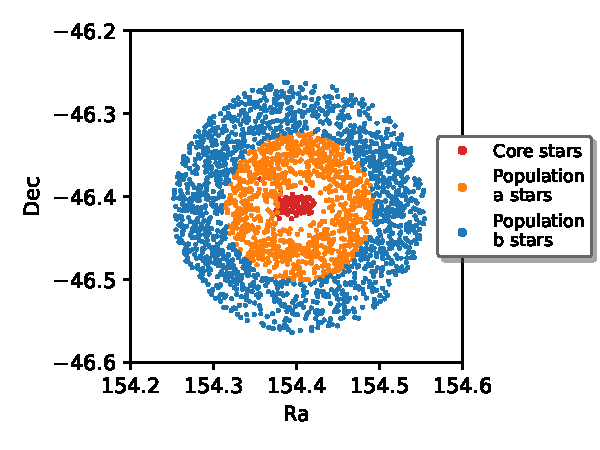
\includegraphics[width=\textwidth]{../Figures/radec}
		\vspace{-7mm}
		\caption{RA/Dec}
		\label{fig:radec}
	\end{subfigure}
	\hfill
	\begin{subfigure}[b]{0.49\textwidth}
		\centering
		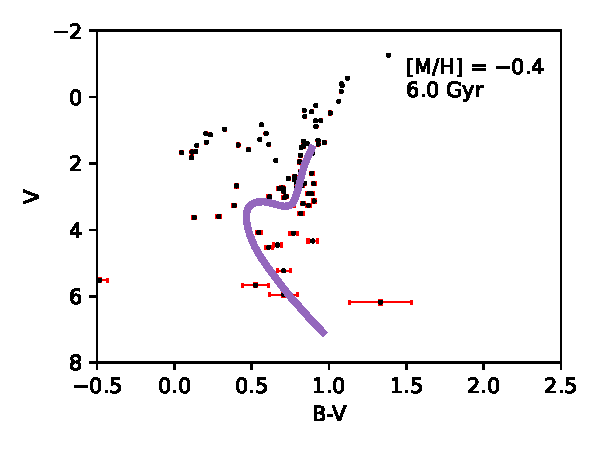
\includegraphics[width=\textwidth]{../Figures/popmanual}
		\vspace{-7mm}
		\caption{Core stars}
		\label{fig:popman}
	\end{subfigure}
	\hfill
	\begin{subfigure}[b]{0.49\textwidth}
		\centering
		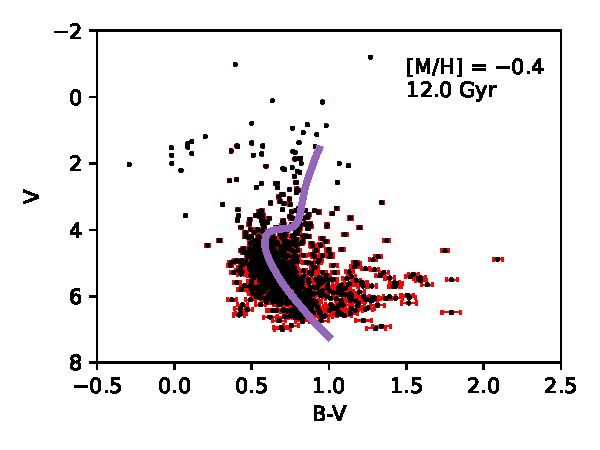
\includegraphics[width=\textwidth]{../Figures/pop1}
		\vspace{-7mm}
		\caption{Population a stars}
		\label{fig:pop1}
	\end{subfigure}
	\hfill
	\begin{subfigure}[b]{0.49\textwidth}
		\centering
		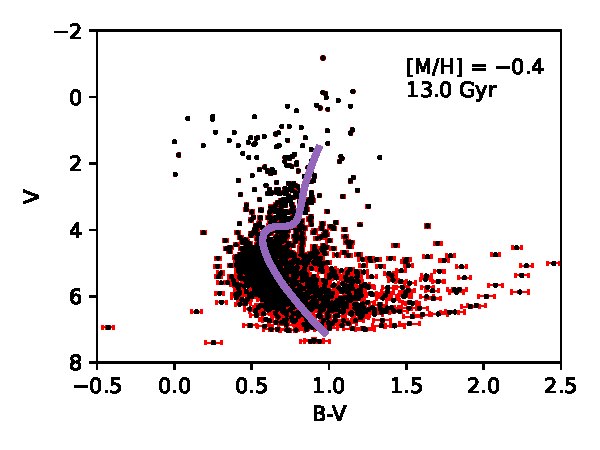
\includegraphics[width=\textwidth]{../Figures/pop2}
		\vspace{-7mm}
		\caption{Population b stars}
		\label{fig:pop2}
	\end{subfigure}
	\caption{The positions of each star in the cluster in RA/Dec (degrees) is shown in \ref{fig:radec} as well as the stars that are in each population. \ref{fig:popman} shows the colour magnitude diagram of the Core stars which has a closest fit isochrone of [M/H] $=-0.4$ and an age of 6.0 Gyr. \ref{fig:pop1} shows the colour magnitude diagram of the Population a stars which are stars within 0.025$^{\circ}$ to 0.09$^{\circ}$ from the centre of the cluster. The fitted isochrone has a [M/H] $=-0.4$ and an age of 13.0 Gyr. \ref{fig:pop2} shows the colour magnitude diagram of Population b stars which are stars that are greater than 0.09$^{\circ}$ from the centre. The fitted isochrone has a [M/H] $=-0.4$ and an age of 12.0 Gyr.}
	\label{fig:populations}
\end{figure}

The populations in Figure \ref{fig:populations} are based on the distance from the centre of the cluster. The method of determining which distance to set each population was done by observing the point where there was a noticeable magnitude difference between the populations.

\section{Discussion}

The age of NGC 3201 found from Figure \ref{fig:iso} is in agreement with \citet{Layden_2003}, who used a similar method, but is in disagreement with metallicity as they have obtained a [M/H] $=-1.72 \pm 0.11$. The reason for this large discrepancy in metallicity are not clear, but it should be noted that the there are more stars past B-V $=1.0$ than in Figure \ref{fig:origin} in their colour magnitude diagram. This could mean larger amounts of low magnitude stars are being recorded in this report than there should be. A reason for this could be due to the automatic detection tool picking up background stars that are not within NGC 3201. The method to determine which isochrone fit to use is not exact, as it realised on visually determining the best fit. A more accurate way of selecting the best isochrone fit would be to used a least squared fitting method which would also allow a more scientific estimate of the uncertainty in the age and metallicity. 

According to \citet{Mackey} classification scheme NGC 3201 would be classified as bulge disk cluster from the metallicity results found in Figure \ref{fig:origin}. This would mean that NGC 3201 has a galactic origin instead of an extragalactic origin.

The automated detection tool was unable to accurately identify stars within the core of the cluster due to the grouping of stars, this meant a manual method of recording the magnitudes was need. Only 80 stars were recorded which cannot give an accurate representation of the entire cluster so any analysis of NGC 3201's age or metallicity based on the manual aperture photometry results is likely to have lots of uncertainty. 

The populations with differing ages in Figure \ref{fig:populations} show that there is an inhomogeneous stellar makeup within NGC 3201. The results show that the stars in the core are younger than the stars in the rest of the cluster. This suggests that NGC 3201 might be the result of two different clusters colliding/merging which makes it hard to categorise in the scheme by \citet{Mackey}. This uncertainty in the origins of NGC 3201 also align with the results found by \citet{god} which suggests that NGC 3201 could have galactic origins instead of extragalactic. This report has found two agreeing results that are in opposition to \citet{Mackey} classification scheme for abnormal clusters. The colour magnitude of NGC 3201 is analysed in Figure \ref{fig:origin} which suggests that NGC 3201 is galactic in origin due to its metallicity which disagrees with \citet{Mackey}. If NGC 3201 is broken down into stellar populations, as shown in Figure \ref{fig:populations}, then more information can be found regarding its origin. This leads to the theory that NGC 3201 was formed by two colliding clusters, which causes the separate population ages in the cluster. 

The data in this report are not plentiful enough to support a concrete result, especially for the core region of the cluster where there was fewer recordings, so there is no strong evidence for the origin of NGC 3201. This means that the classification scheme by \citet{Mackey} works for most clusters but the small number of abnormal clusters like NGC 3201  might need a revision in their classification. The origins of NGC 3201 found in this report are in agreement with \citet{god} but the results of NGC 3201's age and metallicity found in this report have a high uncertainty and unknown validity. Further research needs to be done on methods to more accurately separate the populations in NGC 3201 rather than basing it on the distance from the centre.

\section{Conclusion}

The globular cluster NGC 3201 was analysed using aperture photometry to create a colour magnitude diagram in the B and V filters. An isochrone from \citet{iso} that most closely matched the colour magnitude diagram was determined and the metallicity and age of NGC 3201 was found. From the isochrone the age of NGC 3201 was found to be 12.0 Gyr which is in agreement with \citet{Layden_2003} and the metallicity is $-0.4$ which is in disagreement with both \citet{Layden_2003} and \citet{Mackey} who found it to be roughly $-1.5$. According to the \citet{Mackey} cluster classification scheme, the results in this report would classify NGC 3201 as a bulge disk cluster, with galactic origins, which is in disagreement with \citet{Mackey}. Further analysis of stellar populations within NGC 3201 show that there are groups of stars with different ages which suggests that NGC 3201 was formed by a merger between two previous clusters. This would mean that NGC 3201 would be galactic in origin which is in agreement with \citet{god}. These results cannot prove the origin of NGC 3201 but they can question the validity of the \citet{Mackey} classification scheme when identifying abnormal clusters. Further work needs to be done on more accurately identifying the stellar populations in NGC 3201 rather than taking them from the distance to the centre of the cluster. This would give a better understanding of the origin of NGC 3201. 

\pagebreak
\bibliographystyle{agsm}
\bibliography{Mainref.bib}

\end{document}